% !Mode:: "TeX:UTF-8"

\chapter{原始数据统计性描述、可用性分析和冗余与错误清理}

\section{原数数据分析与统计性描述}

\subsection{用户与基站连接记录数据分析}

哈尔滨市移动平台注册 163,348,433 人次(即电话卡数量),仅 2020 年 1 月 1 日一天,就产生了 1,089,986,353 条连接基站的记录,排除掉 400 开头的虚拟号码、座机号码、企业用物联网卡、IMSI 为 13 位的非个人号码之后,4578524 位个人用户当天产生了 412000435 条约 1.2 TB 的基站连接记录。 其中,每天有至少 100 位用户,在基站之间切换了 1500 次以上,最高能达到 2189 次,平均每位用户日均切换基站 80.0604 次。

\begin{table}[htbp]
    \caption{基站连接信息}
    \vspace{0.5em}\centering\wuhao
    \begin{tabular}{ccccc}
        \toprule[1.5pt]
        变量名 & 数据名称 & 数据类型 & 样例 & 备注 \\
        \midrule[1pt]
        id & 基站 id & string & 3G44 & 基站唯一标识符 \\
        startTime & 开始连接时间 & Long & 1577808000000 & 到 1970-01-01 00:00 的毫秒数 \\
        endTime & 结束连接时间 & Long & 1577958050662 & 意义同上 \\
        \bottomrule[1.5pt]
    \end{tabular}
    \label{tab:cell_con}
\end{table}

数据保存在文件系统基于 HDFS 和 SQL 语句基于 MapReduce 的 Hive 数据库中,数据结构如表 \ref{tab:cell_con} 所示。需要注意的是,由于技术问题,基站 id 并不一定存在于基站基本信息表中(可能非移动公司基站),以及开始和结束连接时间可能为 null 的问题,需要首先对无效的数据进行处理。

\subsection{基站基本信息表分析与描述性统计}

如表 \ref{tab:cell_info} 中所描述的基站基本信息表的数据结构,主要考虑的是基站的唯一标识符 id,以及基站本身的经纬度坐标。

\begin{table}[htbp]
    \caption{基站基本信息表}
    \vspace{0.5em}\centering\wuhao
    \begin{tabular}{ccccc}
        \toprule[1.5pt]
        变量名 & 数据名称 & 数据类型 & 样例 & 备注 \\
        \midrule[1pt]
        id & 基站 id & string & 3G44 & 基站唯一标识符 \\
        lon & 基站经度 & double & 126.624709 & 绕城高速范围 [126.48, 126.83] \\
        lat & 基站维度 & double & 46.770206 & 绕城高速范围 [45.64, 45.86] \\
        \bottomrule[1.5pt]
    \end{tabular}
    \label{tab:cell_info}
\end{table}

基站唯一标识符和用户基站连接记录数据匹配,通过信息表中的经纬度信息,从而得到用户在某一时刻连接的基站的经纬度坐标,则能推算出用户在某时刻的大致位置信息。随机选取一位用户,如图 \ref{fig:track} 表示该用户在一段时间内的基站连接轨迹序列,同时能能够得知该位用户连接某基站(图 \ref{fig:stop} 中红圈标记附近一基站 )3.4 天。

\begin{figure}[ht]
    \centering
    \begin{minipage}[t]{0.49\textwidth}
        \centering
        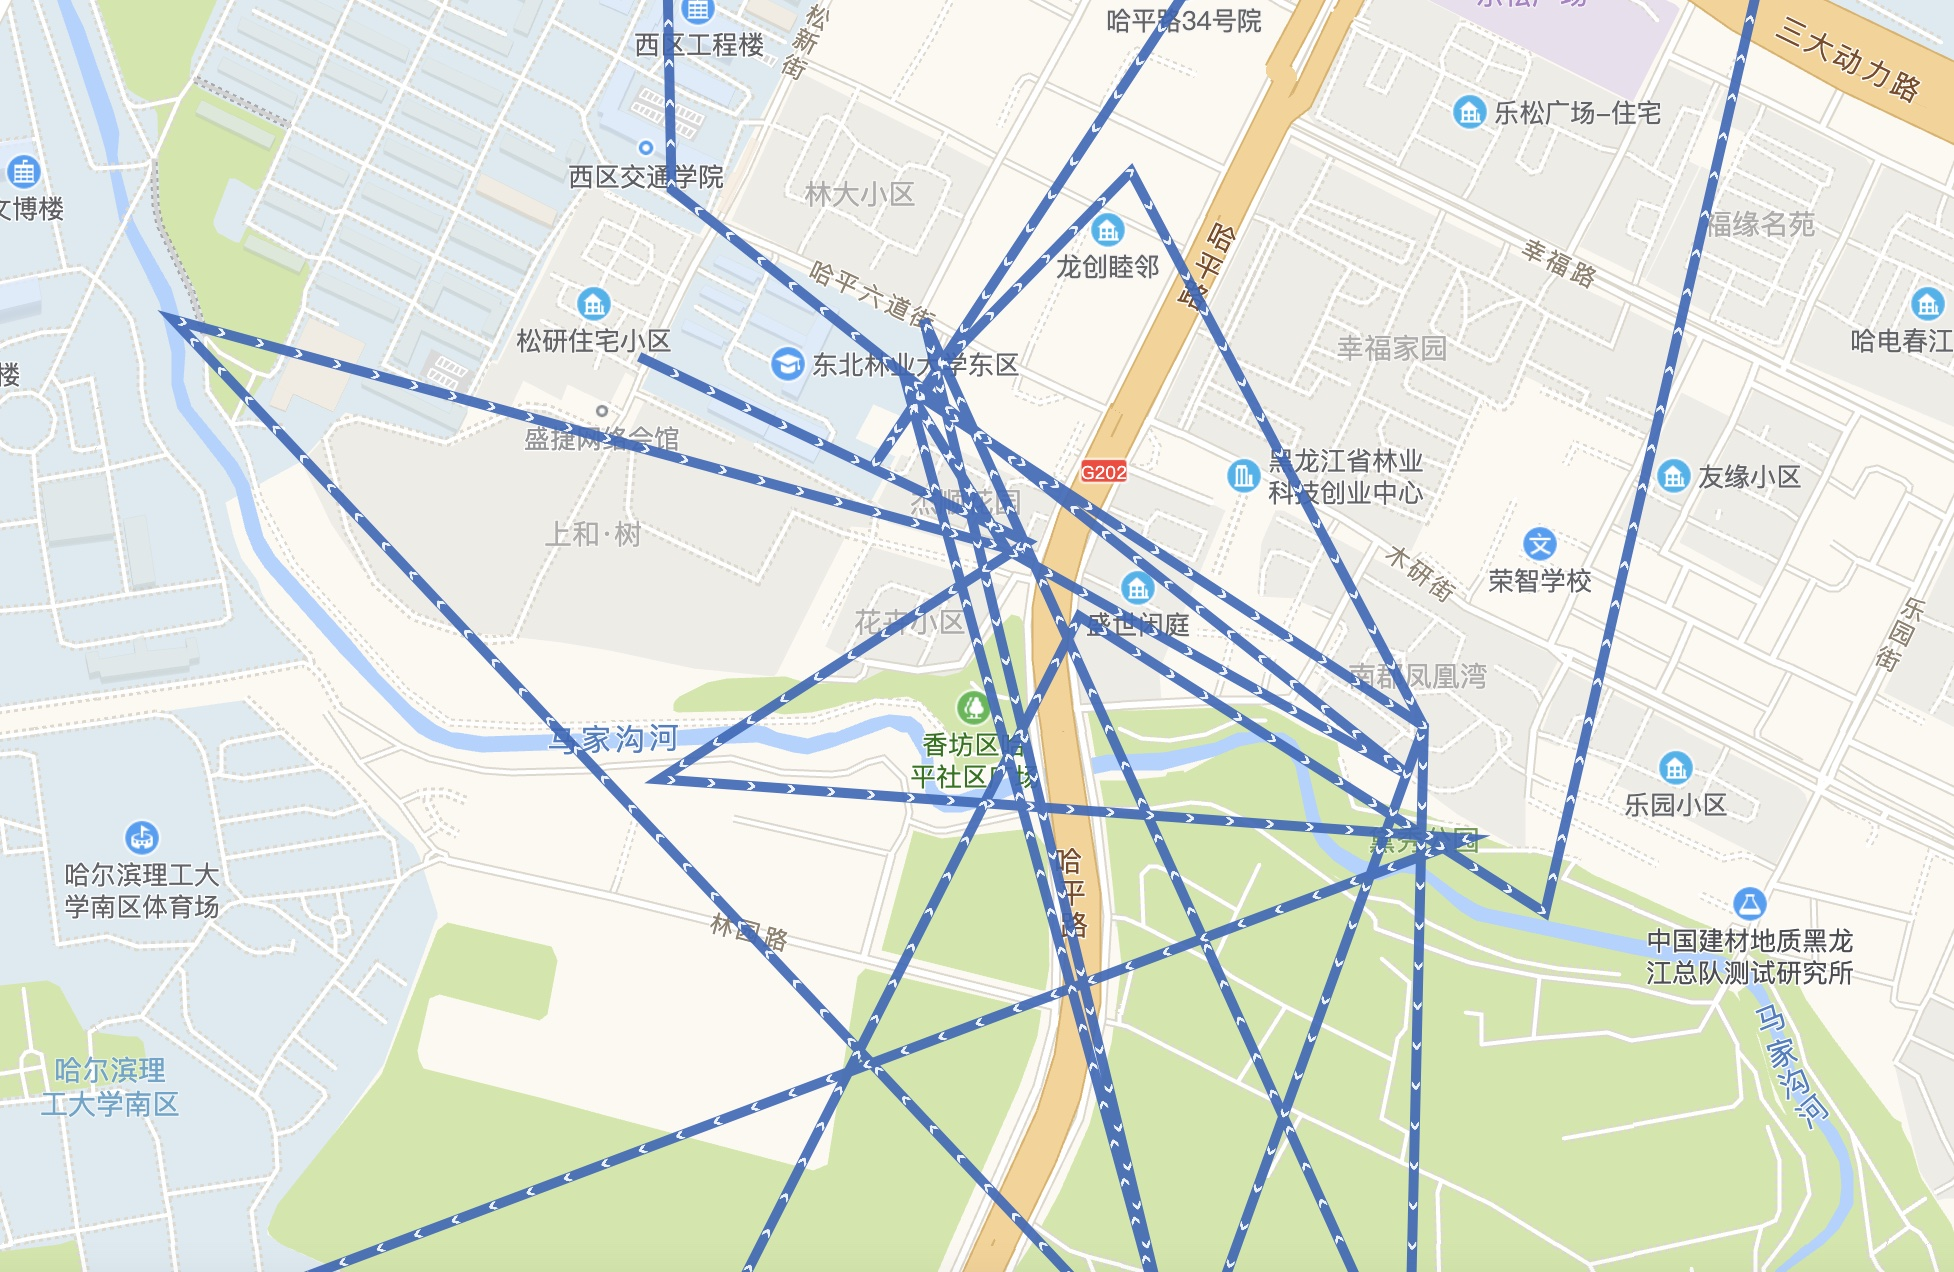
\includegraphics[width = 0.9\textwidth]{track.jpg}
        \caption{基站连接轨迹图}
        \label{fig:track}
    \end{minipage}
    \begin{minipage}[t]{0.49\textwidth}
        \centering
        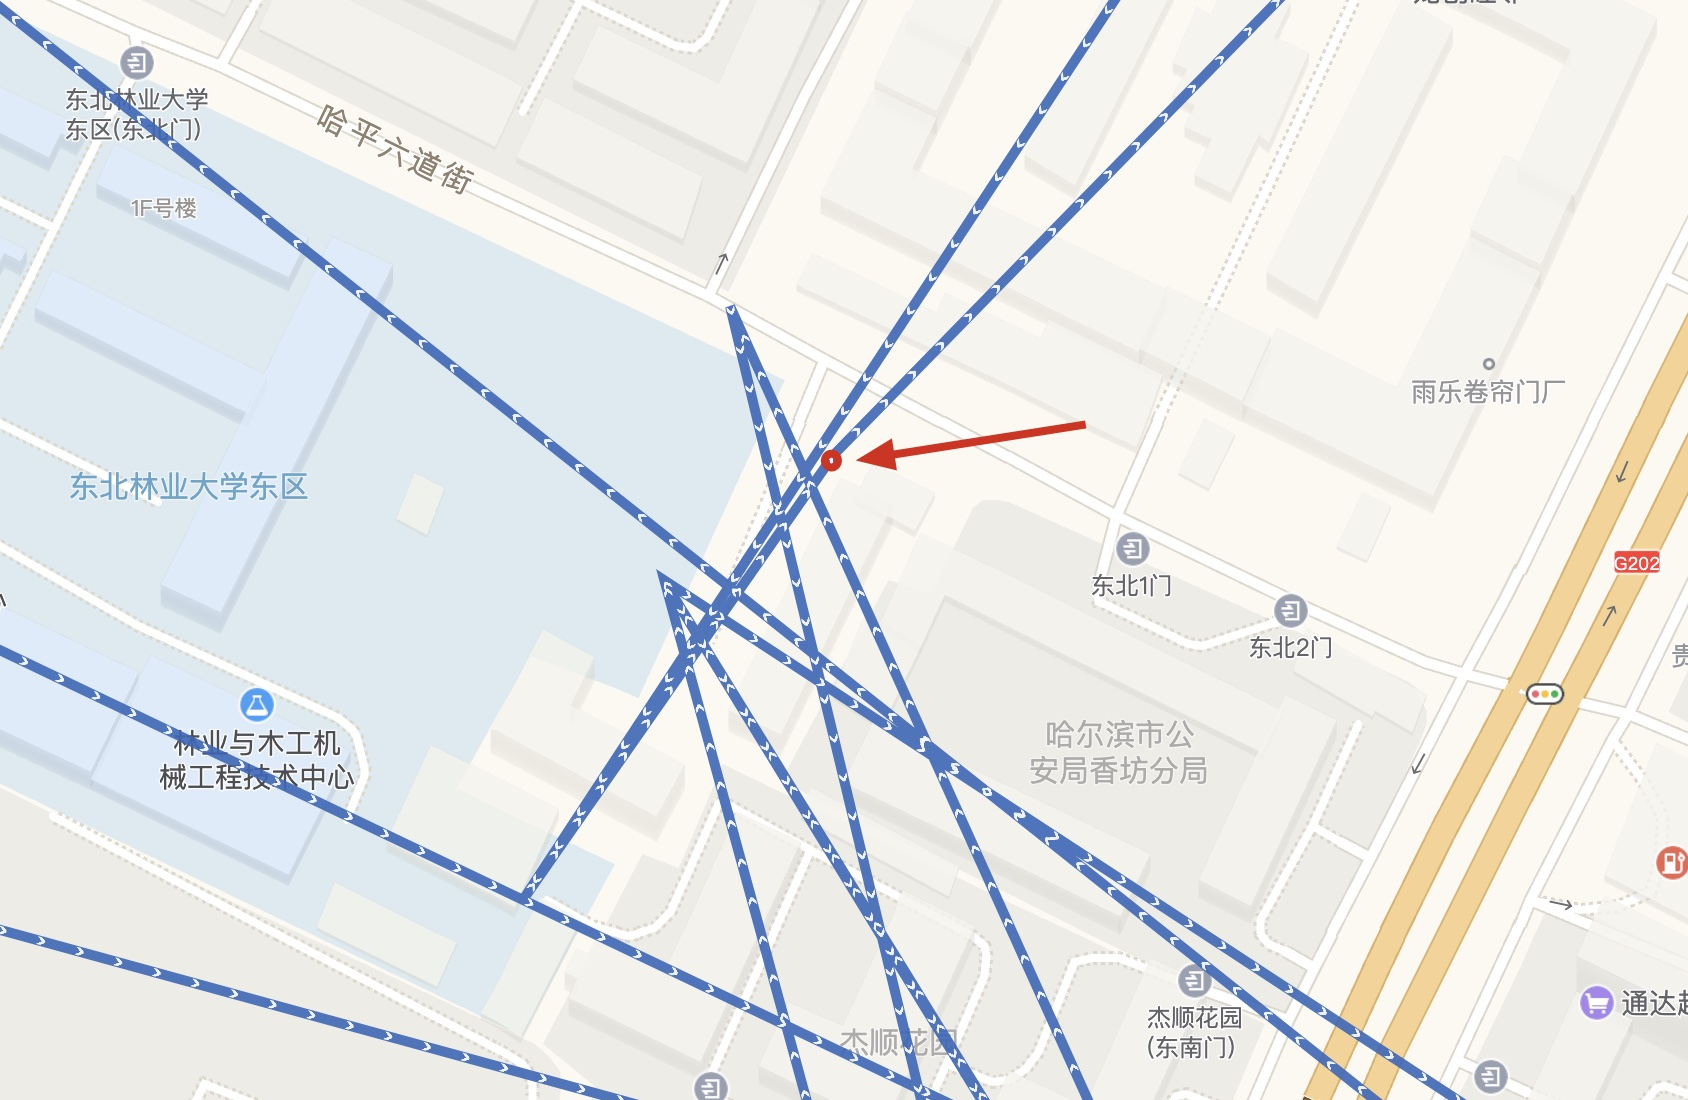
\includegraphics[width = 0.9\textwidth]{stop.jpg}
        \caption{停留地点}
        \label{fig:stop}
    \end{minipage}
\end{figure}

不过由于基站的覆盖面积实在是太大,如图 \ref{fig:cell_con} 中所示,2020 年 1 月 1 日,研究人员本人一天只前往过教化街附近的学生十八公寓、学苑楼、诚意楼,但是却能连接到学校西北部哈尔滨银行附近的一个基站长达 2.1 个小时,以及曲线街(图中未显示,连接次数排名第 5)移动营业厅附近一基站一小时左右。基站的连接轨迹并不能准确的表达用户的真实位置,后面几章将会如何利用基站经纬度坐标推算用户驻留点偏好。

\begin{figure}[ht]
    \centering
    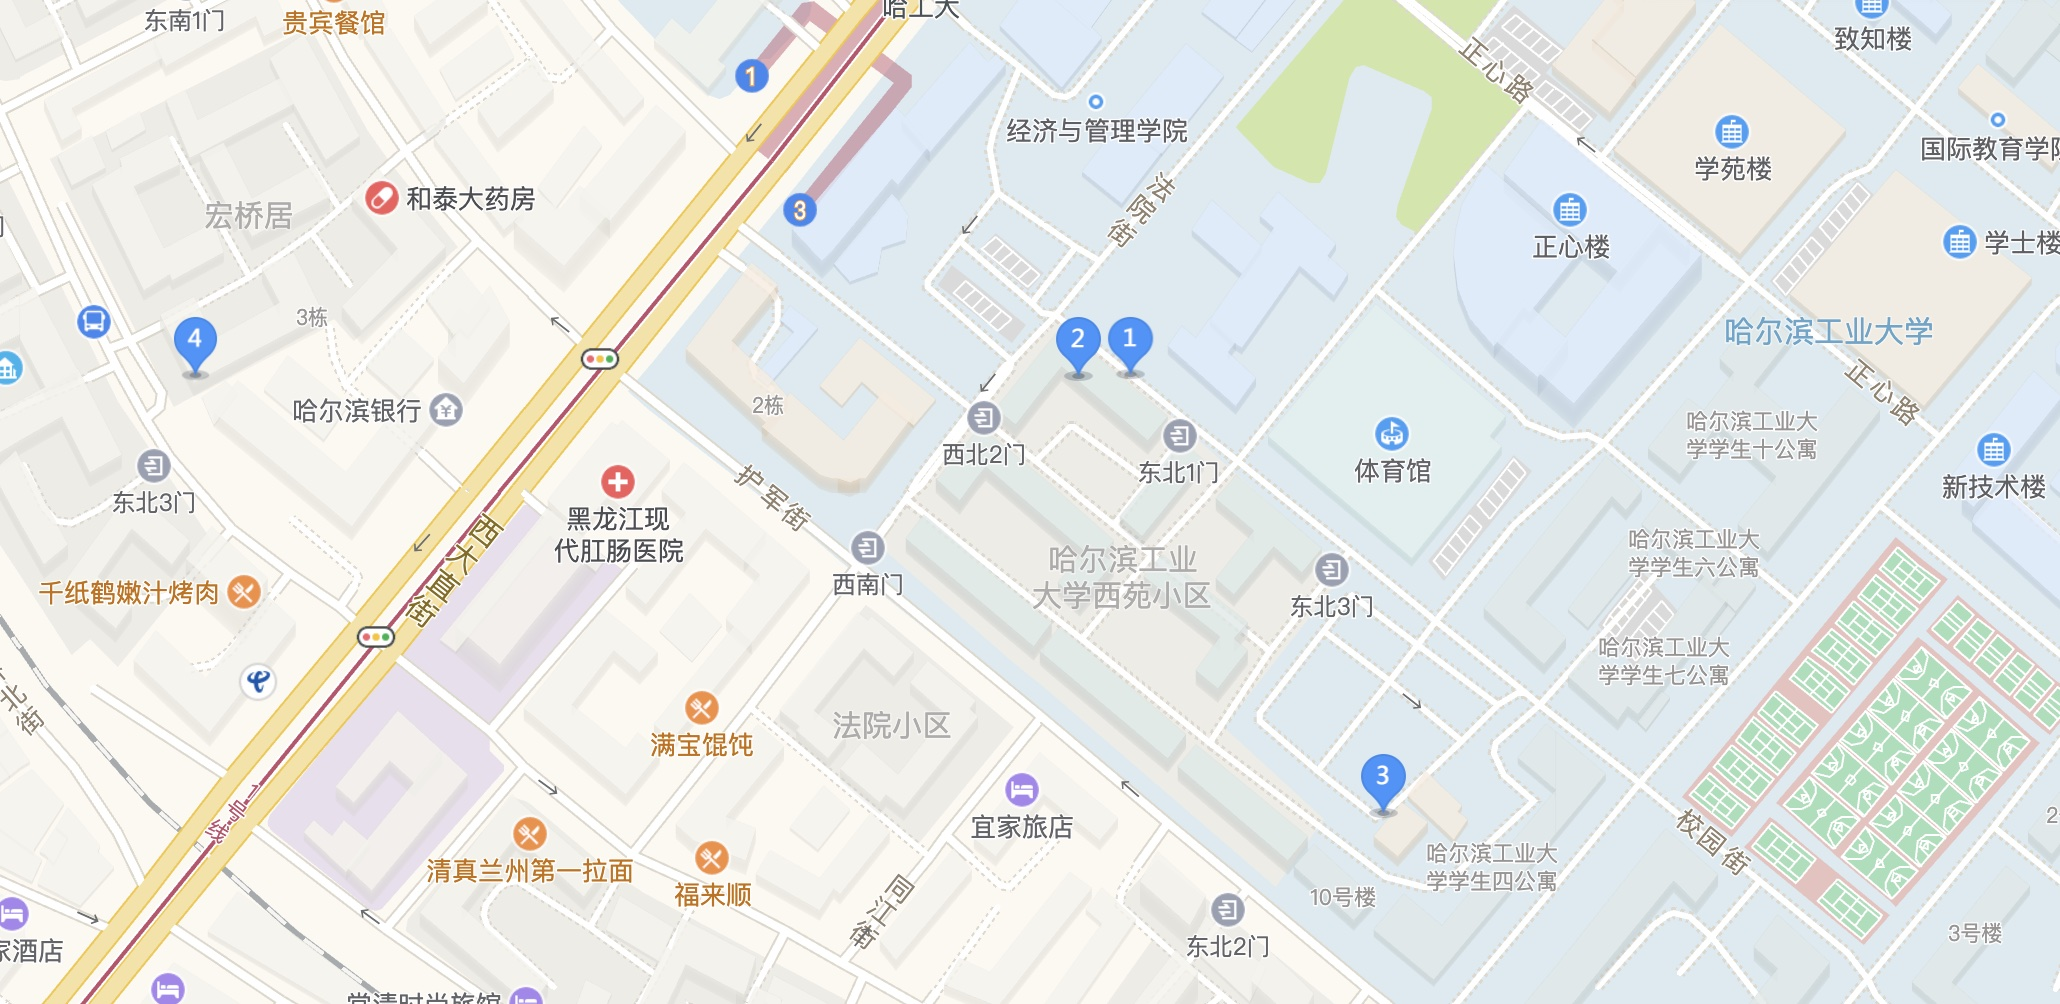
\includegraphics[width = 0.8\textwidth]{cell_con.jpg}
    \caption{连接的最多的基站}
    \label{fig:cell_con}
\end{figure}

\section{哈尔滨市 POI 兴趣点爬取、处理和描述分析}

首先从高德地图上爬取哈尔滨市所有的 POI 兴趣点的相关信息,包括 POI 兴趣点的序号、名称、类型(如购物中心、餐厅、体育场、学校等)、POI 经纬度信息,数据结构如表 \ref{tab:poi_info} 所示。

\begin{table}[htbp]
    \caption{哈尔滨市 POI 兴趣点数据结构}
    \vspace{0.5em}\centering\wuhao
    \begin{tabular}{ccccc}
        \toprule[1.5pt]
        变量名 & 数据名称 & 数据类型 & 样例 & 备注 \\
        \midrule[1pt]
        id & 兴趣点 id & int & 123 & 兴趣点唯一标识符 \\
        name & 兴趣点名称 & string & 远大购物中心 & 名称描述 \\
        type & 兴趣点类型 & string & 购物中心 & 类型描述 \\
        lon & POI 位置经度 & double & 126.556693 & \\
        lat & POI 位置维度 & double & 45.738066 & \\
        \bottomrule[1.5pt]
    \end{tabular}
    \label{tab:poi_info}
\end{table}

\begin{figure}[htbp]
    \centering
    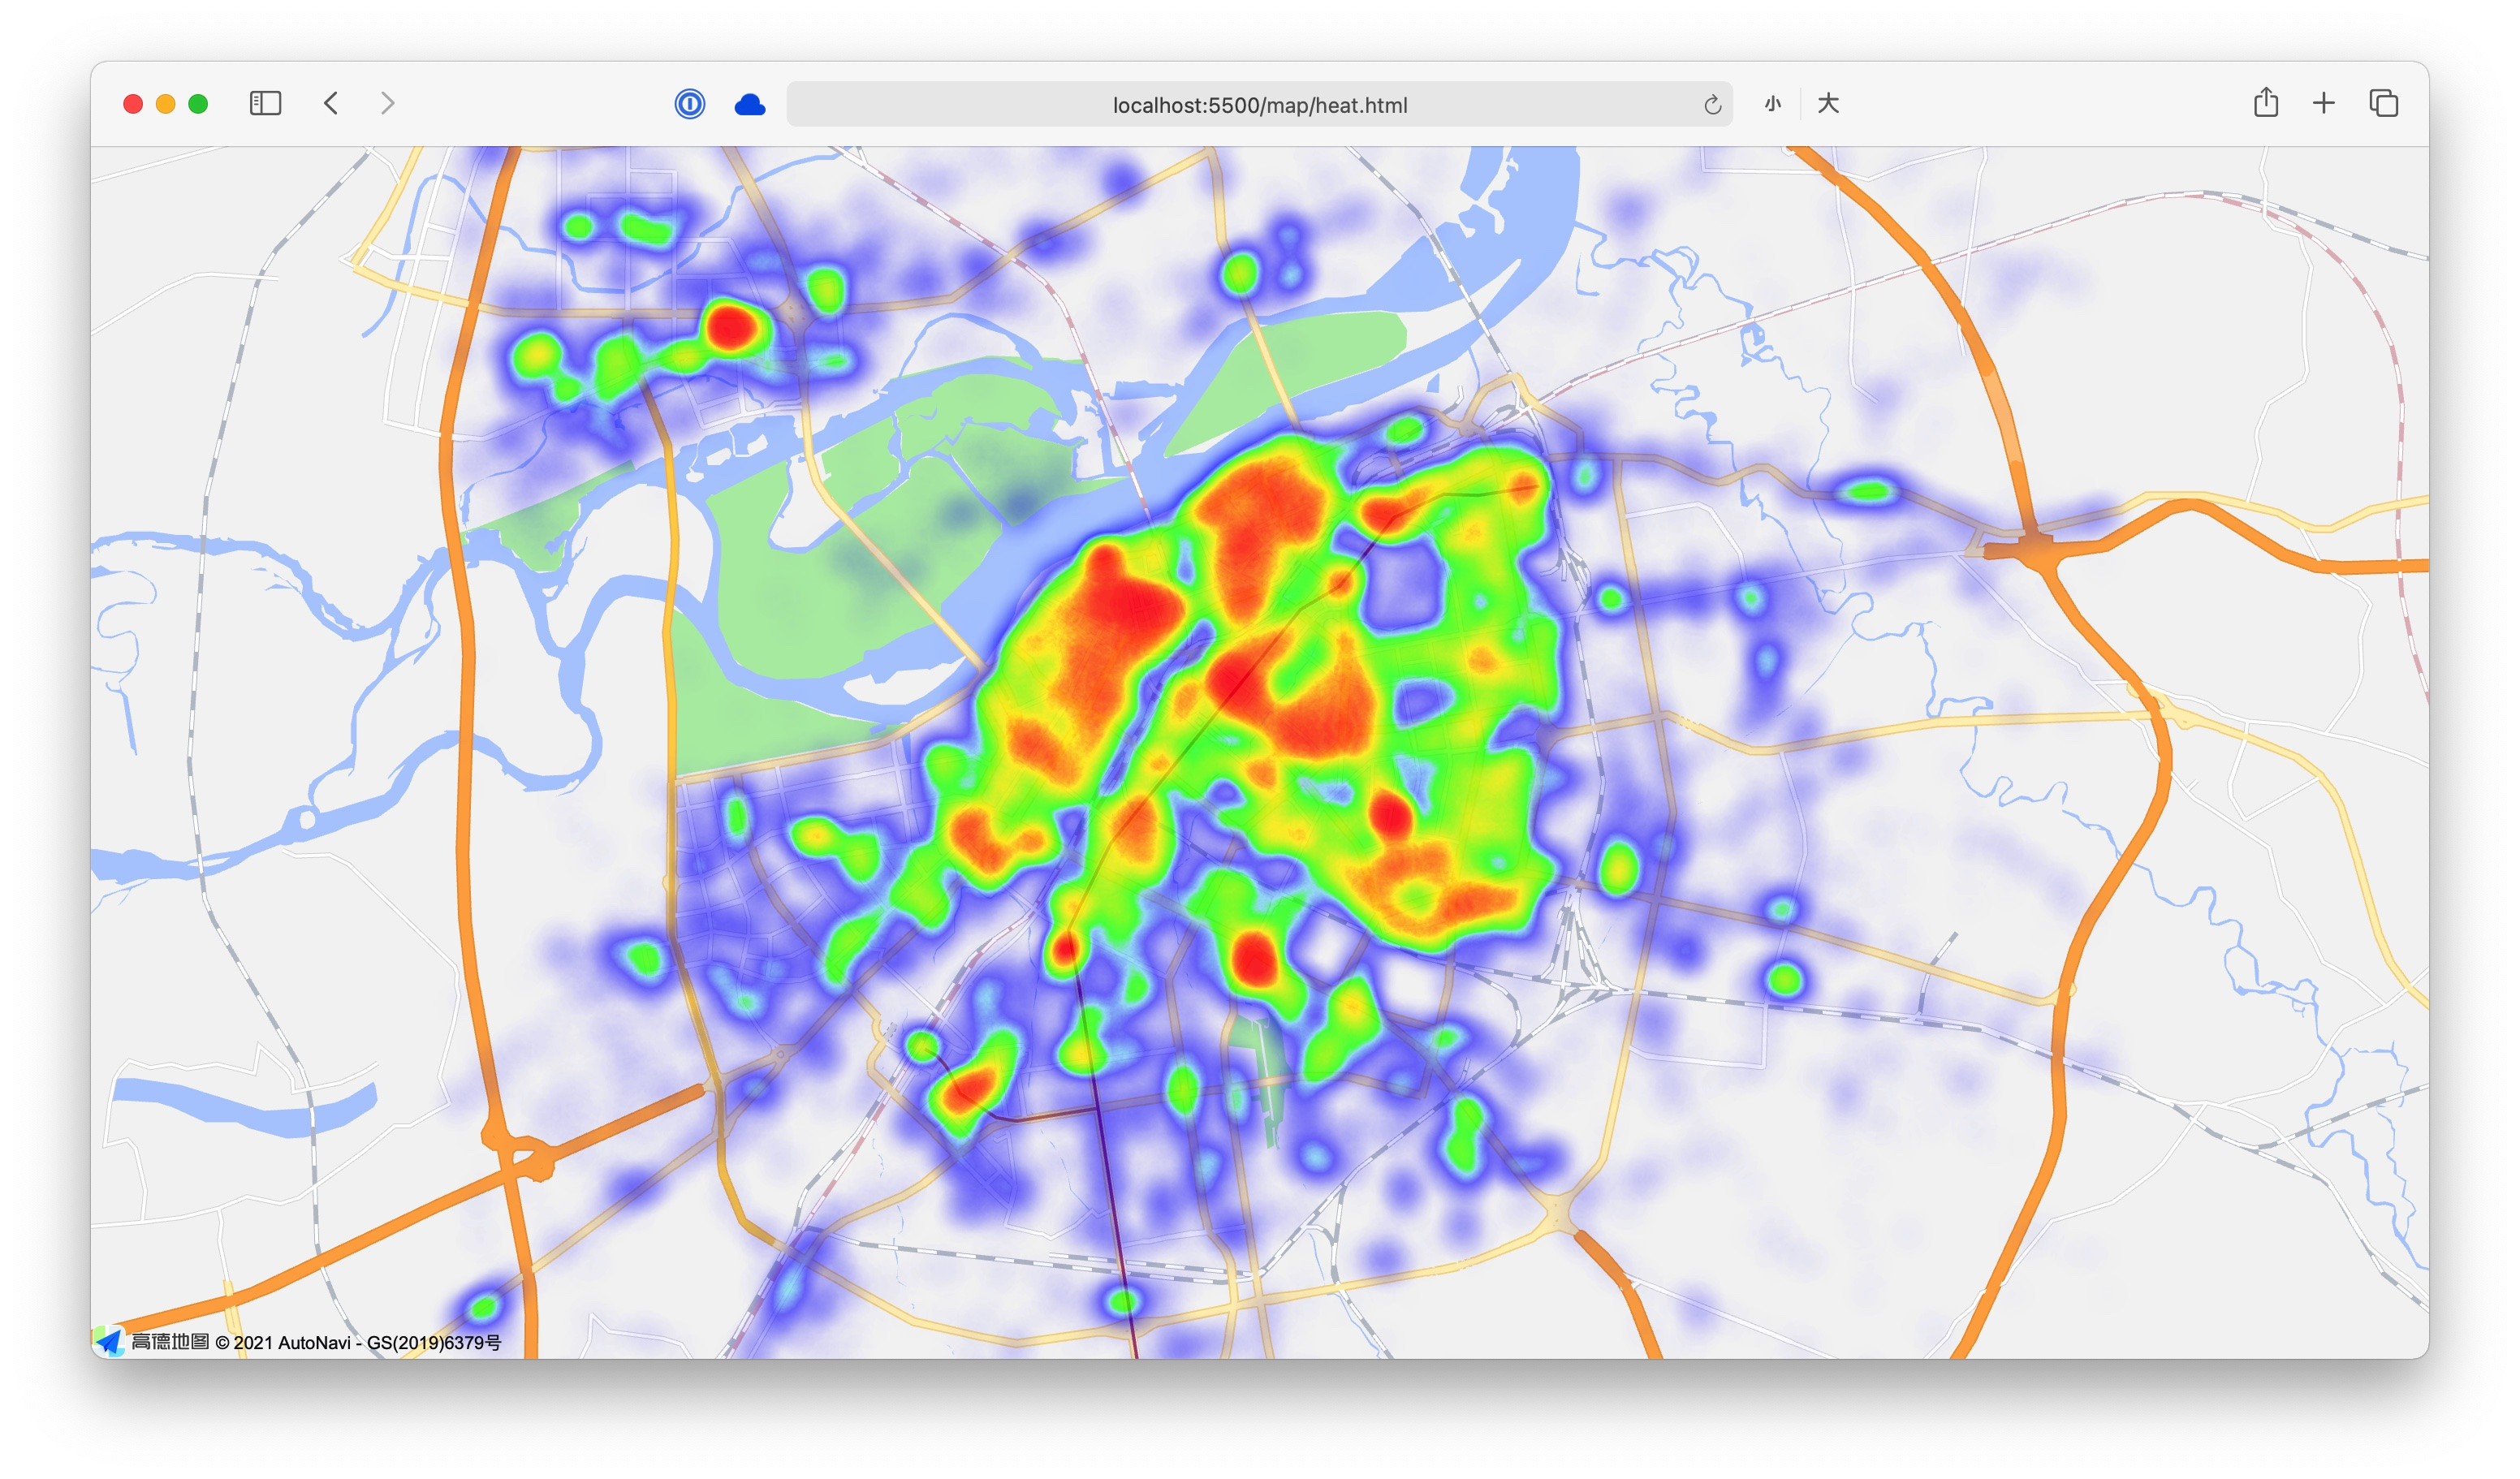
\includegraphics[width = 0.9\textwidth]{poi_gen.jpg}
    \caption{全市 POI 兴趣点分布热力图}
    \label{fig:poi_gen}
\end{figure}

一共 477932 个 POI 兴趣点,每个兴趣点间隔最小小于 1m(经纬度描述相同),最远一千米以上。基站分布如图 \ref{fig:poi_gen} 所示。根据用户基站连接数据统计数据、POI 分布热力图所描述,用户在环城高速以内的活动更为活跃同时用以描述用户移动语义的 POI 兴趣点也更多,所以我们选择哈尔滨市绕城高速以内的市区进行分析,如图 \ref{fig:harbin_raocheng} 所示。

\begin{figure}[htbp]
    \centering
    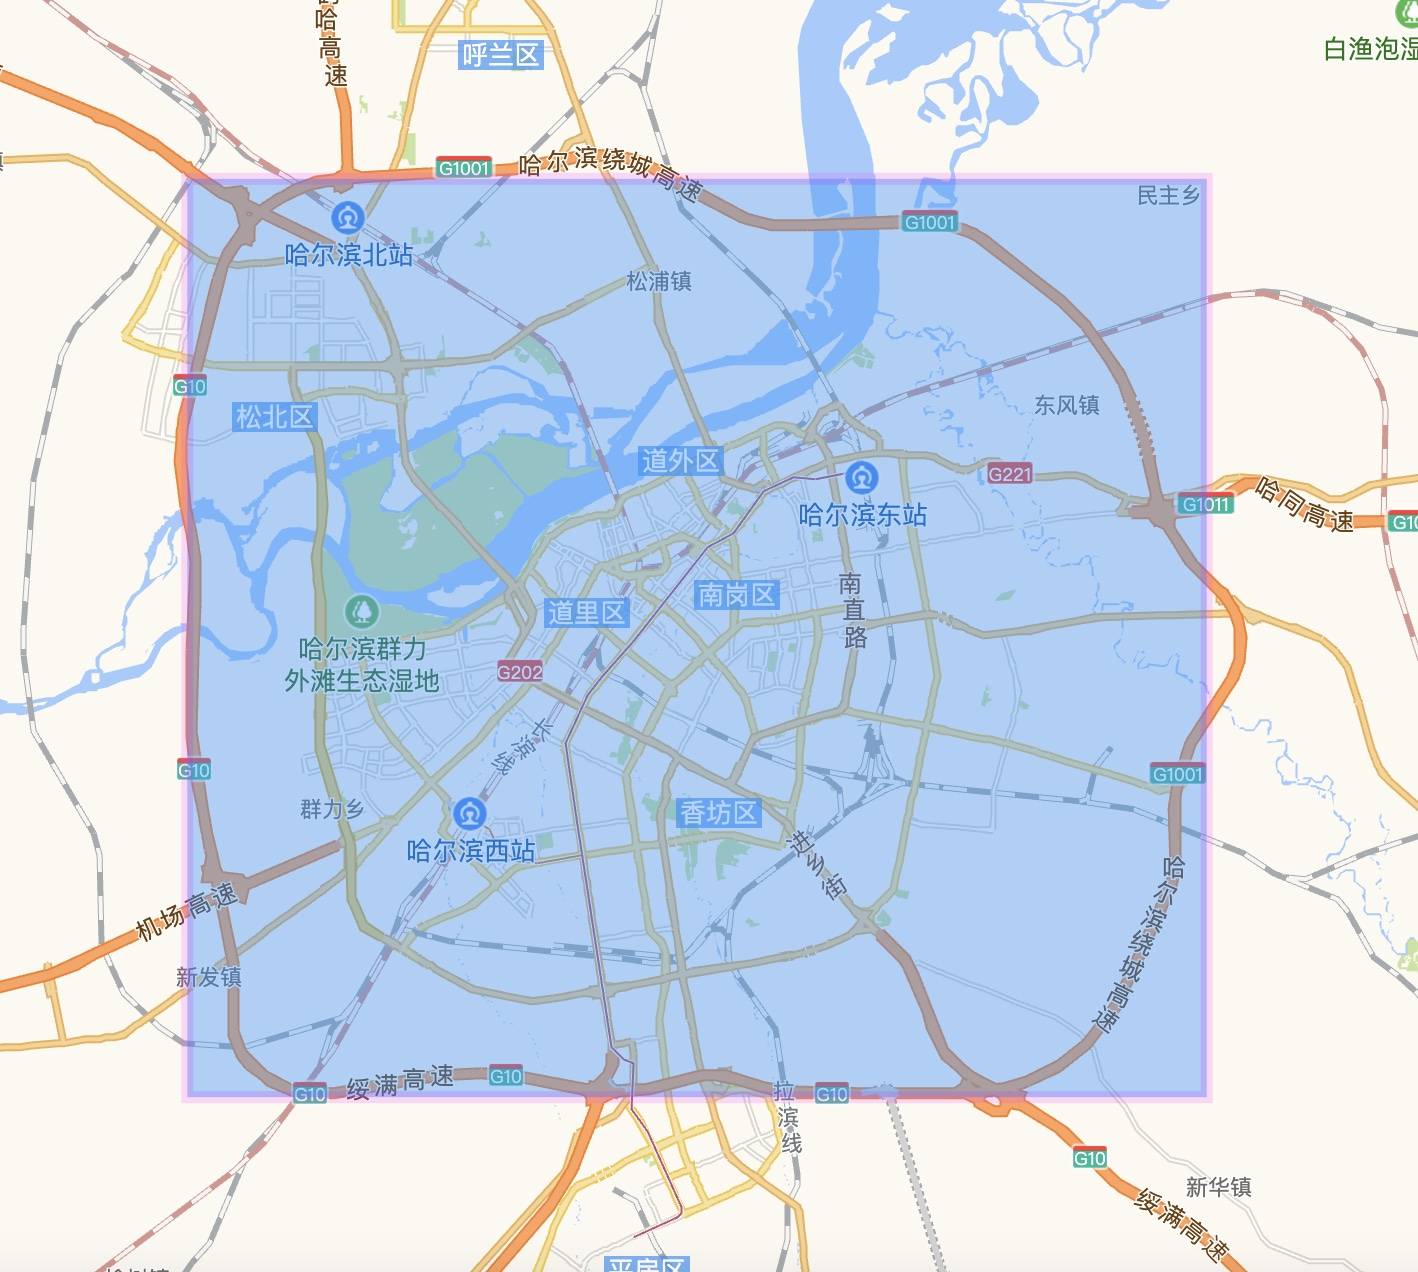
\includegraphics[width = 0.5\textwidth]{district.jpg}
    \caption{哈尔滨市绕城高速范围}
    \label{fig:harbin_raocheng}
\end{figure}

\section{用户手机应用使用流量记录表分析}

\begin{table}[htbp]
    \caption{哈尔滨市用户各个基站的分时流量数据表}
    \vspace{0.5em}\centering\wuhao
    \begin{tabular}{ccccc}
        \toprule[1.5pt]
        变量名 & 数据名称 & 数据类型 & 样例 & 备注 \\
        \midrule[1pt]
        date & 日期 & string & 20200615 & \\
        user\_id & 用户 id & string & 13912345678 & 用户唯一标识符 \\
        app\_id & 手机应用 id & string & C946 & 手机应用唯一标识符 \\
        app\_name & 应用名称 & string & 腾讯视频 & \\
        lon & POI 位置经度 & double & 126.556693 & \\
        lat & POI 位置维度 & double & 45.738066 & \\
        data & 流量数据(单位 B) & int & 578 & 每个小时一个数据,共 8 列 \\
        \bottomrule[1.5pt]
    \end{tabular}
    \label{tab:app_use}
\end{table}

由于 4G 网络在中国的快速铺开,网民飞速增长的同时,移动端应用的使用也越来越频繁,哈尔滨市用户日手机应用流量使用记录数据表可达 600MB,包括记录的日期,用户 id(即手机号码),应用 id(应用商店中应用的唯一标识符),应用名称,基站经纬度,以及从 0 时到 23 时的流量使用数据(单位 Byte),数据结构如表 \ref{tab:app_use} 所示。

爬取手机应用商店中的数据(此处选择华为手机应用商店),经统计,一共 4563 款下载量明显的手机应用,数据维度过多,此处选择使用手机应用的二级类型数据进行降维处理,转为统计用户在某个时间段对某类应用的偏好。爬取的应用数据中包含:如为了和用户应用使用信息表匹配的应用唯一标识符 id,应用一级类型,应用二级类型,下载量,评分等,数据结构如表 \ref{tab:app_info} 所示。

\begin{table}[htbp]
    \caption{手机应用基本信息表}
    \vspace{0.5em}\centering\wuhao
    \begin{tabular}{ccccc}
        \toprule[1.5pt]
        变量名 & 数据名称 & 数据类型 & 样例 & 备注 \\
        \midrule[1pt]
        app\_id & 手机应用 id & string & C946 & 手机应用唯一标识符 \\
        type\_1 & 应用一级类型 & string & 社交软件 & \\
        type\_2 & 应用二级类型 & string & 聊天 & \\
        download & 下载量 & int & 50912769 & 截止到爬取时 \\
        score & 评分 & double & 3.5 & 满分 5 分 \\
        \bottomrule[1.5pt]
    \end{tabular}
    \label{tab:app_info}
\end{table}

\section{用户通话和短信使用记录数据表分析}

为了描述用户的社交地位和偏好,还需要使用用户通话和短信使用记录的相关数据,通话数据包括统计的月份,拨出手机号码,接收手机号码,对端归属地,通话时长,通话次数,通话天数等,数据结构如表 \ref{tab:call_data} 所示。

\begin{table}[htbp]
    \caption{手机应用基本信息表}
    \vspace{0.5em}\centering\wuhao
    \begin{tabular}{ccccc}
        \toprule[1.5pt]
        变量名 & 数据名称 & 数据类型 & 单位 \\
        \midrule[1pt]
        stat\_mon & 统计月份 & string & \\
        serv\_no & 手机号码 & string & \\
        opp\_serv\_no & 对端号码 & string & \\
        opp\_type & 对端类型 & string & \\
        opp\_region\_code & 对端归属地 & string & \\
        call\_dur & 通话时长 & long & 秒 \\
        calling\_dur & 通话时长(主叫) & long & 秒 \\
        called\_dur & 通话时长(被叫) & long & 秒 \\
        call\_cnt & 通话次数 & long & 次 \\
        calling\_cnt & 通话次数(主叫) & long & 次 \\
        called\_cnt & 通话次数(被叫) & long & 次 \\
        busy\_call\_cnt & 忙时通话次数 & long & 次 \\
        idle\_call\_cnt & 闲时通话次数 & long & 次 \\
        busy\_dur & 忙时通话时长 & long & 分钟 \\
        idle\_dur & 闲时通话时长 & long & 分钟 \\
        weekday\_sum\_call\_cnt & 工作日通话次数 & long & 次 \\
        weekday\_work\_sum\_call\_cnt & 工作日上班时间通话次数 & long & 次 \\
        weekday\_offwork\_sum\_call\_cnt & 工作日非上班时间通话次数 & long & 次 \\
        weekend\_sum\_call\_cnt & 周末通话次数 & long & 次 \\
        weekday\_sum\_call\_dur & 工作日通话时长 & long & 分钟 \\
        weekend\_sum\_call\_dur & 周末通话时长 & long & 分钟 \\
        call\_days & 通话天数 & long & 天 \\
        first\_call\_date & 末次通话时间 & string & \\
        last\_call\_date & 首次通话时间 & string & \\
        \bottomrule[1.5pt]
    \end{tabular}
    \label{tab:call_data}
\end{table}

同理,用户点对点短信记录信息表中包含统计日期、用户类型、发送方号码、发送方归属区号、接收方号码、接收方归属区号、短信条数等信息,数据结构如表 \ref{tab:msg_data} 所示。

\begin{table}[htbp]
    \caption{手机应用基本信息表}
    \vspace{0.5em}\centering\wuhao
    \begin{tabular}{ccccc}
        \toprule[1.5pt]
        变量名 & 数据名称 & 数据类型 \\
        \midrule[1pt]
        stats\_mon & 统计月份 & string \\
        user\_type & 用户类型 & string \\
        send\_serv\_no & 发送方手机号码 & string \\
        home\_city\_code & 发送方归属区号 & string \\
        reci\_serv\_no & 接收方手机号码 & string \\
        opp\_city\_code & 接收方归属区号 & string \\
        gms\_count & 短信条数 & long \\
        \bottomrule[1.5pt]
    \end{tabular}
    \label{tab:msg_data}
\end{table}

\section{本章小结}

本章通过对原始数据的统计性描述和分析,首先确定了可用的数据库和能用以分析用户画像的数据的结构,统计数据中可能有误和缺失的信息,做好标记用以支持之后的正式处理中采用剔除或默认值的办法替换原值;同时统计数量大小和有效数据范围,如每日信息数量、统计区域范围(哈尔滨市绕城高速)等,为后续小样本的计算模型测试提供理论基础;

\chapter{哈尔滨市城区 POI 兴趣点数据获分析和栅格化街区聚类分析}

\section{哈尔滨市城区 POI 兴趣点数据具体分析}

为了能够描述用户的移动语义(即用户前往目的地的原因),同时由于基站的覆盖面积过于宽广,并不能直接将基站的位置认为是用户的目的位置,文献 \cite{phithakkitnukoon_activity-aware_2010}\cite{dashdorj_semantic_2018} 中 Phithakkinukoon 和 Dashjor 指出,用户的移动语义是由某一个范围内的兴趣点的分布情况决定的,如果得知了该区块中各类型兴趣点的分布,那么我们就能大致推算前往该区域的用户的目的。

如图 \ref{fig:hit_poi},为哈尔滨工业大学一校区周边 POI 兴趣点分布地图,若一个区域中分布着教学楼、公寓、食堂、超市等兴趣点,

\begin{figure}[htbp]
    \centering
    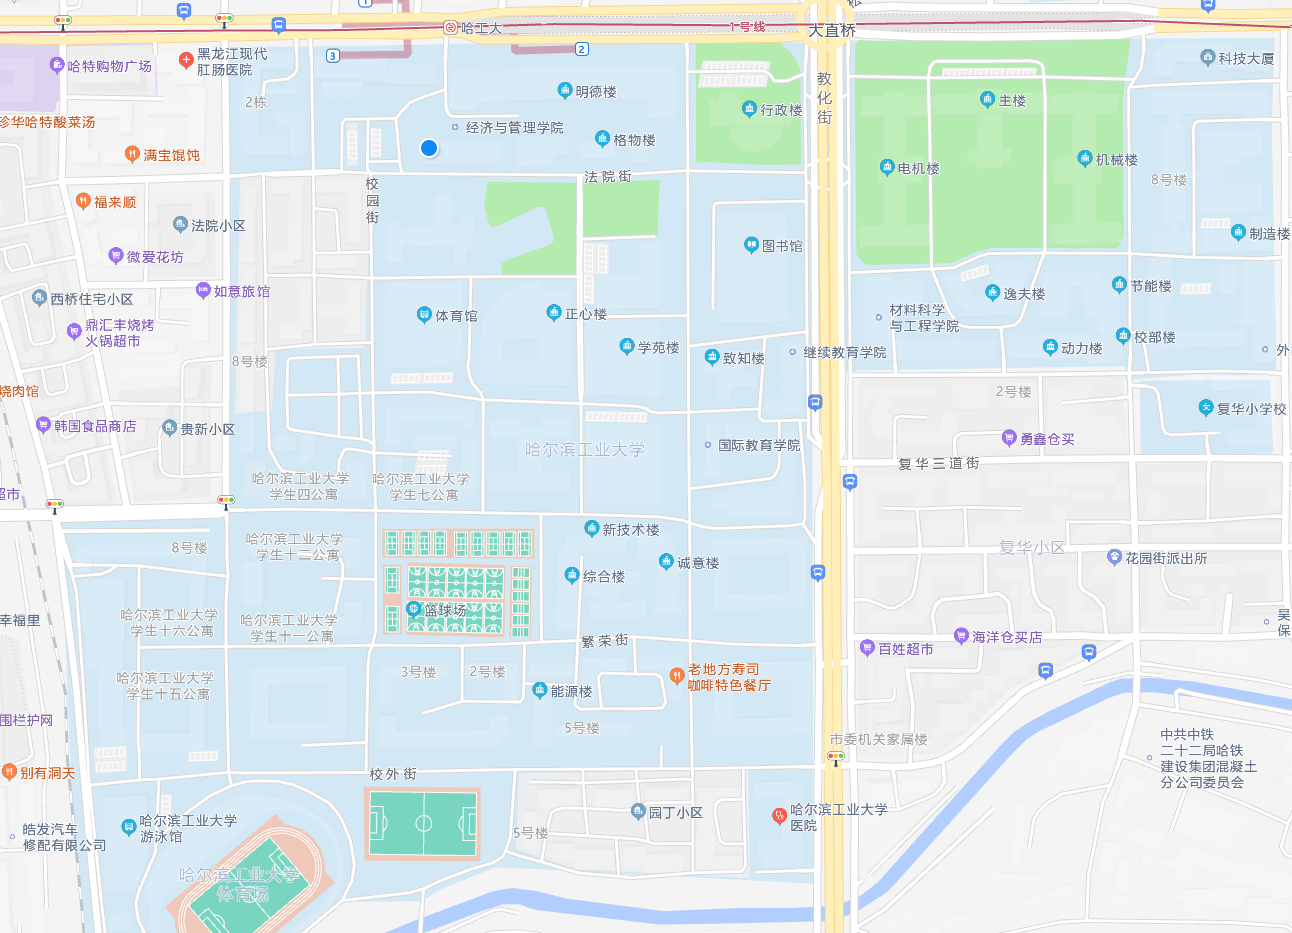
\includegraphics[width = 0.9\textwidth]{hit_poi.png}
    \caption{哈尔滨工业大学一校区周边 POI 兴趣点分布图}
    \label{fig:hit_poi}
\end{figure}

\section{基于路网和栅格化的功能区聚类分析模型对比}

\section{功能区的栅格化参数的分析和对比}

\section{本章小结}

\chapter{大数据领域下聚类方法的对比和在哈尔滨城市功能区的聚类结果分析}

\section{DBSCAN 聚类算法概述和分析}

\section{K-Means 聚类算法概述}

K-Means 算法的思想非常简单,对于样本集,按照距离划分为若干个簇,让簇内距离最小化,簇间距离最大化。如果有集合 $G$,假设划分的簇为\\ $(U_1, U_2, \dots, U_m)$,则我们的目标则是最小化误差 $E$:

$$
E = \sum_{i=1}^{m}\sum_{x \in U_{i}} ||x - \mu_{i}||^{2}_{2}
$$

其中,$\mu_{i}$ 是每个簇的质心,通常是一个均值向量。传统的算法通常是随机选择 $k$ 质心(即要分成多少类),经常会根据先验经验做一个 $k$ 值选择,对于每一次迭代,求每个点到每个质心的距离,最小距离则为改簇,重复迭代,直到质心没有变化。

\section{K-Means 初始质心选择优化 K-Means++ 算法}

在最基础的 K-Means 聚类中,最初的质心的选择通常是随机选择,而在 K-Means++ 中,则是优化最初的质心选择,优化策略也比较简单,方法如下:

\begin{enumerate}
    \item 随机选择一个点作为第一个质心 $\mu_{1}$;
    \item 对于寻找第 $i$ 个质心,则计算数据集中没有作为质心的点,分别到前 $i - 1$ 个质心的最小距离 $D_{j} = \min(Distance(j, i))$;
    \item 有概率的选择第 $i$ 个质心,原则是 $D_{j}$ 越大的点作为第 $i$ 个质心的概率越大;
    \item 重复,选出 $k$ 个质心;
\end{enumerate}

但是 K-Means 的优化只能优化迭代的次数,而 K-Means 的算法复杂度是 $O(MNKD)$,$N$ 为样本数量,$K$ 为聚类个数,$D$ 为数据维度,$M$ 与数据集本身的分布情况和中心点有关 \emph{此处有引用},K-Means++ 的优化对于本研究 4 百万的原数样本数量来说,并不是特别的高效。

\section{大样本优化 Mini Batch K-Means 算法}

在上上节所述的 K-Means 的传统算法中,每次迭代都需要计算数据集中每个节点到质心的距离,当数据量达到 10 万以上时,即使加上诸如 elkan K-Means 优化\emph{此处有引用} 也无法应付。此时,就要用到 Mini Batch K-Means 算法。

如同字面意思,Mini Batch,原理十分简单,从数据集中随机抽取一部分样本,做普通的 K-Means 聚类,得到的质心就被认定为最终的质心。由于 $N$ 缩小的很快,导致算法每次跌打的速度大大加快,当然,精度也会降低,不过经过证明 \emph{此处有引用},仍然在我们的可接受范围内,而且通常会进行多次 Mini Batch K-Means 聚类,选择其中最优的聚类结果。

如图  的一次 K-Means 与 Mini Batch K-Means 对比,二者的运行时间相差两倍多,但最终的结果差异确非常小,图中第三张(Difference)的粉色错误点。

\section{哈尔滨市功能区聚类结果分析和展示}

\section{本章小结}

\chapter{大数据系统不同计算框架的分析与对比}

\chapter{基于手机信令数据的用户驻留点、手机应用偏好以及社交地位分析}

\chapter{基于驻留点、应用偏好和社交地位分析结果的用户职住特征分析}

% Local Variables:
% TeX-master: "../main"
% TeX-engine: xetex
% End:
